% Created 2025-05-20 Tue 13:14
% Intended LaTeX compiler: pdflatex
\documentclass{article}


%%%%%%%% ICML 2025 EXAMPLE LATEX SUBMISSION FILE %%%%%%%%%%%%%%%%%
\usepackage[T1]{fontenc}
% Recommended, but optional, packages for figures and better typesetting:
\usepackage{microtype}
\usepackage{graphicx}
\usepackage{subfigure}
\usepackage{booktabs} % for professional tables

% hyperref makes hyperlinks in the resulting PDF.
% If your build breaks (sometimes temporarily if a hyperlink spans a page)
% please comment out the following usepackage line and replace
% \usepackage{icml2025} with \usepackage[nohyperref]{icml2025} above.
\usepackage{hyperref}


% Attempt to make hyperref and algorithmic work together better:
\newcommand{\theHalgorithm}{\arabic{algorithm}}

% Use the following line for the initial blind version submitted for review:
\usepackage[accepted]{style/icml2025}

% If accepted, instead use the following line for the camera-ready submission:
%% \usepackage[accepted]{style/icml2025}

% For theorems and such
\usepackage{amsmath}
\usepackage{amssymb}
\usepackage{mathtools}
\usepackage{amsthm}


% if you use cleveref..
\usepackage[capitalize,noabbrev]{cleveref}
%%%%%%%%%%%%%%%%%%%%%%%%%%%%%%%%
% THEOREMS
%%%%%%%%%%%%%%%%%%%%%%%%%%%%%%%%
\theoremstyle{plain}
\newtheorem{theorem}{Theorem}[section]
\newtheorem{proposition}[theorem]{Proposition}
\newtheorem{lemma}[theorem]{Lemma}
\newtheorem{corollary}[theorem]{Corollary}
\theoremstyle{definition}
\newtheorem{definition}[theorem]{Definition}
\newtheorem{assumption}[theorem]{Assumption}
\theoremstyle{remark}
\newtheorem{remark}[theorem]{Remark}

% Todonotes is useful during development; simply uncomment the next line
%    and comment out the line below the next line to turn off comments
%\usepackage[disable,textsize=tiny]{todonotes}
\usepackage[textsize=tiny]{todonotes}

% The \icmltitle you define below is probably too long as a header.
% Therefore, a short form for the running title is supplied here:
\icmltitlerunning{Test short title ICML 2025}


\usepackage[inkscapelatex=false]{svg}
\date{}
\title{}
\hypersetup{
 pdfauthor={Alan Munoz},
 pdftitle={},
 pdfkeywords={},
 pdfsubject={},
 pdfcreator={Emacs 30.1 (Org mode 9.7.11)}, 
 pdflang={English}}
\usepackage{natbib}
\begin{document}

\twocolumn[
\icmltitle{cp\_measure: API-first feature extraction for image-based profiling workflows}

% It is OKAY to include author information, even for blind
% submissions: the style file will automatically remove it for you
% unless you've provided the [accepted] option to the icml2025
% package.

% List of affiliations: The first argument should be a (short)
% identifier you will use later to specify author affiliations
% Academic affiliations should list Department, University, City, Region, Country
% Industry affiliations should list Company, City, Region, Country

% You can specify symbols, otherwise they are numbered in order.
% Ideally, you should not use this facility. Affiliations will be numbered
% in order of appearance and this is the preferred way.
\icmlsetsymbol{equal}{*}

\begin{icmlauthorlist}
\icmlauthor{Al\'an F. Mu\~{n}oz}{broad}
\icmlauthor{Tim Treis}{hh,broad}
\icmlauthor{Alexandr A. Kalinin}{broad}
\icmlauthor{Shatavisha Dasgupta}{broad}
\icmlauthor{Fabian Theis}{hh}
\icmlauthor{Anne E. Carpenter}{broad}
\icmlauthor{Shantanu Singh}{broad}
\end{icmlauthorlist}

\icmlaffiliation{broad}{Broad Institute of MIT and Harvard, United States}
\icmlaffiliation{hh}{Institute of Computational Biology, Helmholtz Zentrum München, Germany}

\icmlcorrespondingauthor{Al\'an F. Mu\~{n}oz}{amunozgo@broadinstitute.org}
\icmlcorrespondingauthor{Shantanu Singh}{shantanu@broadinstitute.org}

% You may provide any keywords that you
% find helpful for describing your paper; these are used to populate
% the "keywords" metadata in the PDF but will not be shown in the document
\icmlkeywords{Machine Learning, ICML}

\vskip 0.3in
]

% this must go after the closing bracket ] following \twocolumn[ ...

% This command actually creates the footnote in the first column
% listing the affiliations and the copyright notice.
% The command takes one argument, which is text to display at the start of the footnote.
% The \icmlEqualContribution command is standard text for equal contribution.
% Remove it (just {}) if you do not need this facility.

\printAffiliationsAndNotice{}  % leave blank if no need to mention equal contribution
% \printAffiliationsAndNotice{\icmlEqualContribution} % otherwise use the standard text.

\begin{abstract}
Biological image analysis has traditionally focused on measuring specific visual properties of interest for cells or other entities. A complementary paradigm gaining increasing traction is image-based profiling - quantifying many distinct visual features to form comprehensive profiles where patterns of changes show biological properties. While current tools like CellProfiler can generate these feature sets, they pose significant barriers to automated and reproducible analyses, hindering ML workflows. Here we introduce cp\_measure, a Python library that extracts CellProfiler's core measurement capabilities into a modular, API-first tool designed for programmatic feature extraction. We demonstrate that cp\_measure features retain high fidelity with CellProfiler features while enabling seamless integration with the scientific Python ecosystem. Through applications to 3D astrocyte imaging and spatial transcriptomics, we showcase how cp\_measure enables reproducible, automated image-based profiling pipelines that scale effectively for machine learning applications in computational biology.
\end{abstract}

\section{Introduction}
\label{sec:org4c9ba67}
High throughput screening of biological phenomena via complex modalities, such as RNA sequencing, is prohibitively expensive, therefore microscopy is an efficient first step. Through microscopy, modern biologists use a wide array of fluorescence dyes or proteins to observe the location and distribution of cells, organelles, and other components. Nowadays, quantification of biological images is standard, with software often identifying regions of interest (such as cells) and extracting features that represent these regions, such as intensity distributions.

Image-based profiling--also termed morphological profiling--is a technique of measuring an array of shape and intensity features for a population of biological objects, such as cells. These features are fed into statistical or machine learning methods to identify biologically meaningful patterns. One of its biggest applications is drug discovery, where scientists leverage microscopy's low acquisition cost and high throughput to accomplish many goals, such as grouping genes by function, identifying chemical compounds that target a protein, and predicting toxicity of drug candidates \citep{sealDecadeSystematicReview2024}. 

\begin{figure}[htbp]
\centering
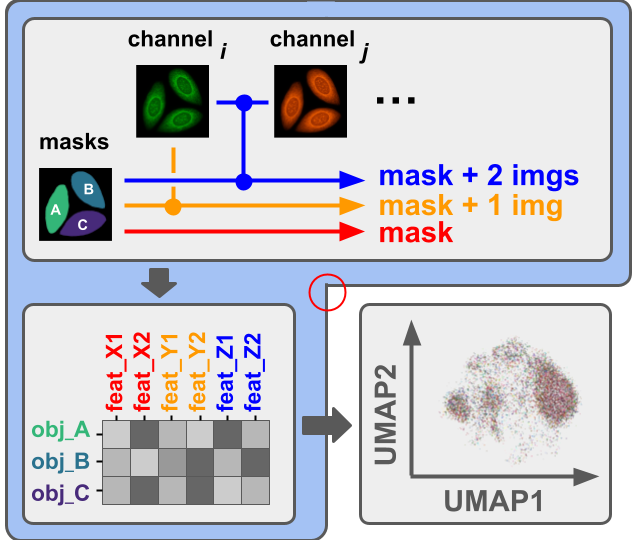
\includegraphics[width=.99\linewidth]{./figs/fig_1_tmp.png}
\caption{\label{fig:overview}cp\_measure generates features from images by using information in every region of interest ("object"). It can featurize the pairwise combination of all the available channels (colours) and objects. The resultant matrices represent the entire experiment and can be studied using statistical, machine, and deep learning methods.}
\end{figure}

\subsection{The current state of bioimage analysis}
\label{sec:org8f5b33d}
The most widely used software for processing high-throughput biological images is CellProfiler \citep{stirlingCellProfiler4Improvements2021}. It can be used by experimental biologists with scant programming experience, for whom it has been a boon. By contrast, it may not suit the needs of computer-savvy scientists building high throughput pipelines comprised of multiple tools. CellProfiler is ideal for creating and iteratively adapting manually-defined workflows; for low-customization high-throughput analyses such as extracting features for image-based profiles, however, certain aspects become a hindrance. For example, complementing CellProfiler with other image analysis tools is a struggle, as building plug-ins to add functionality is a time and effort-consuming challenge that requires an understanding of its interfaces. Lastly, CellProfiler depends on many Python and Java packages, increasing the likelihood of dependency conflicts. Containers mitigate this problem, but not without increased complexity and caveats.

Alternative tools can extract features for image-based profiles, such as scikit-image \citep{waltScikitimageImageProcessing2014}, ScaleFex, or SpaCR \citep{comoletHighlyEfficientScalable2024,einarolafssonSpaCr2025} . However, these come with constraints: Given that their implementation is completely independent from CellProfiler, they do not produce the same feature set, precluding matching to existing datasets, such as those in the Cell Painting Gallery \cite{weisbartCellPaintingGallery2024,fayRxRx3PhenomicsMap2023}. Moreover, a common problem is that these tools enforce a structure for the input data, such as determined hierarchical file structures, which require significant wrangling with the data before processing a single image. Some alternatives, such as ScaleFex, are designed for cloud usage, neglecting a significant number of cases where local compute suffices. 

\subsection{Engineered features in the era of deep learning}
\label{sec:org9dc3dfa}
An alternative to extracting a defined set of engineered features is to instead use a pretrained deep-learning model to extract features. Results are mixed, with suitably-trained deep learning networks usually outperforming engineered features \cite{lafargeCapturingSingleCellPhenotypic2019,moshkovLearningRepresentationsImagebased2022,chowPredictingDrugPolypharmacology2022,wolfSCANPYLargescaleSinglecell2018}, but not always \cite{tangMorphologicalProfilingDrug2024,kimSelfsupervisionAdvancesMorphological2023}. Training a deep learning model to be a good feature extractor takes significant hands-on and compute time, and often requires appropriate training images. Compared to engineered features, deep learning approaches may pose a higher barrier of entry, as most models require either annotated data or a large and high-quality dataset, in addition to having access to a GPU. Foundational models aim to lower this barrier, but can fail to generalize well for out-of-distribution data (data which differs sufficiently from the training datasets) \cite{azadFoundationalModelsMedical2023}. Generally deep learning-based feature extraction takes less wall-clock time than CellProfiler does (provided GPU compute is available); however, the features are not obviously interpretable and require specialized techniques for biologists to attempt to understand patterns of changes in image-based profiles, which is not always successful \citep{liChallengesOpportunitiesBioimage2023}.  Unlike learned features, whose interpretation requires complex methods like counterfactual techniques or attention maps, most engineered features have a mathematical definition that is faster to calculate and easier to translate into biological concepts, such as the colocalisation of two proteins \cite{garcia-fossaInterpretingImagebasedProfiles2023}.

In summary, while deep learning-based features have some advantages in some contexts, and while tools to extract engineered features exist, there remains a need for a modular tool that can extract interpretable features while readily integrating with computational workflows to achieve reproducible data analyses, whether locally or in the cloud. We thus believe that there is the need for a readily-integrated feature extraction tool aimed at generalist and high throughput problems not being solved by the current software ecosystem. With all this in mind, we developed cp\_measure.


\section{Extracting interpretable features}
\label{sec:org61842b5}
The library cp\_measure branches off the CellProfiler codebase, adapted to include calculations for all features of an image-based profiling pipeline, while removing the user interface and anything else non-essential to the task. Measurements are defined as a collection of related features, following CellProfiler's nomenclature, and are categorized based on three kinds of input: One object (producing features such as area and eccentricity), one object + one imaging channel (these can be used to extract such measurements as intensity, texture), one object + multiple channels (e.g., for Manders correlations between intensity values across channels).

By isolating the feature calculations from the graphical interface and orchestration components, we aimed to make them accessible to the data science community while improving reusability, testability and extensibility. This reduces the amount of time and human effort required to integrate featurization into existing and new pipelines, while still retaining the standard set of features available for multiple public datasets.

%First, we demonstrated the validity and capabilities of cp\_measure in cases that would normally require image analysis knowledge and a considerable amount of time. First, we validate cp\_measure features versus CellProfiler results with a subset of the JUMP dataset \citep{chandrasekaranJUMPCellPainting2023}. Then we showcase cases in which cp\_measure is a more practical choice to process microscopy data: First 3D images of astrocytes and then spatial transcriptomics. These use-cases demonstrate its widespread suitability for different types of problems. 
\subsection{Reproducing CellProfiler measurements}
\label{sec:org09b0cd2}

\begin{figure}[htbp]
\centering
\includesvg[width=.9\linewidth]{./figs/jump_r2_examples}
\caption{\label{fig:cp_vs_cpmeasure}cp\_measure features match their CellProfiler analogs. \textbf{Left panel.} Representative examples comparing CellProfiler feature values (x-axis) to cp\_measure's (y-axis), generated using matching pairs of masks and images. \textbf{Right panel.} \(R^2\) value of a linear fit for each individual feature, comparing cp\_measure to CellProfiler.}
\end{figure}

We first tested whether cp\_measure features match the original CellProfiler features, for a representative set of 300 images. These correspond to 150 perturbations from the JUMP Cell Painting dataset \citep{chandrasekaranJUMPCellPainting2023}, selecting a representative subset of the most significant phenotypes for each feature. We segmented images to delineate the cells and nuclei using CellProfiler, providing object masks (regions of interest) to CellProfiler and to cp\_measure for feature extraction. Next, we applied cp\_measure on these masks and the original images. Finally, we mapped the features from cp\_measure to CellProfiler and calculated a linear fit for each matched feature, plus the \(R^2\) value, indicating how well the correlation fits a linear slope.

We find that most features had an $R^2$ correlation larger than 90\% (Figure \ref{fig:cp_vs_cpmeasure}). We examined several individual features, typically finding straight lines demonstrating the recapitulation of features from our implementation. For a small set of features, some data points fall off the diagonal, which hint that some edge cases are treated differently by either tool; we plan to investigate these further as part of a larger project to implement unit testing in CellProfiler. These results indicate that cp\_measure is not likely to produce massively different profiles than those calculated by CellProfiler.
\subsection{Results}
\label{sec:orge5b5c6b}
\subsubsection{Astrocyte 3D nuclei data}
\label{sec:org447090b}

To demonstrate its ease of use and the value of interpretable features, we next tested cp\_measure in a classification workflow. We processed 433 three-dimensional (3D) images of astrocyte nuclei containing 831 nuclei \citep{kalinin3DCellNuclear2018}. We preprocessed the profiles following standard procedures \citep{caicedoDataanalysisStrategiesImagebased2017}. Then, we trained a Gradient Boosting classifier to identify the day in which the image of any given cell was acquired, which corresponds to the extent of maturation of the cells. We achieved 87\% classification accuracy in the testing dataset. Using the image-based profiles, we identified which features distinguish cells based on the time at which the image was taken. Finally, we calculated the SHAP values \citep{sundararajanManyShapleyValues2020} to get a better understanding of the effects of the drugs on the cells.

\begin{figure}[htbp]
\centering
\includesvg[width=.9\linewidth]{./figs/example_shap.svg}
\caption{\label{fig:astrocytes}\textbf{Top panel.} Example pair of astrocyte nuclei image and masks. The 3D images were projected over the z-axis, taking the maximum value across the z-stack. \textbf{Bottom panel.} SHAP values of the most important features for classifying the day of differentiation (out of three days). Each point represents a single 3D image containing multiple nuclei, the magnitude of SHAP values indicate how important those features are for the classifier. Features are ranked by importance, with individual SHAP values shown for the top features and the summed impact shown for the remaining 267 features shown as a single aggregated value. Shape features refer to the nucleus and intensity features refer to the DNA staining. The test data accuracy is shown in bold.}
\end{figure}

Figure \ref{fig:astrocytes} shows an example image and its corresponding object masks alongside the Shapley values of a classifier trained on our features. The minor axis length of the nuclei increases over the course of the experiment, implying that nuclei become wider - an expected phenotypic change that cp\_measure was able to uncover.
\subsubsection{Spatial transcriptomics}
\label{sec:org5711d86}
A key advantage of providing these features as a stand-alone Python package is their ease of integration into diverse analytical workflows, which otherwise would require substantial adaptation to the standard CellProfiler environment. The recent proliferation of black-box foundation models trained solely on morphological data highlights morphology as a highly informative and predictive modality. However, the feature vectors produced by these models are typically not interpretable, preventing direct biological assessment. In contrast, classical morphological features yield explicit, interpretable readouts -- for instance, the co-localization of fluorescent markers -- facilitating clear biological interpretations.

To demonstrate this utility, we integrated our cp\_measure-based feature extraction into the widely used spatial analysis library Squidpy \citep{pallaSquidpyScalableFramework2022}. Being stand-alone allowed seamless incorporation into workflows powered by the robust SpatialData \citep{marconatoSpatialDataOpenUniversal2025} framework underlying Squidpy. Because spatial datasets often comprise significantly more cells per field-of-view (FOV) than conventional microscopy screenings -- up to approximately 100,000 cells-traditional software typically cannot process these large images without cropping, which introduces boundary artefacts. Leveraging the modular design of cp\_measure, we parallelized feature extraction at the single-cell level, streaming batches of cells across computational cores. This approach enables efficient computation even on large-scale datasets, a feat not achievable with standard CellProfiler software.

To further illustrate the value of morphological features, we evaluated their impact on cell-type prediction tasks using spatial transcriptomics data. This application is particularly compelling, as current spatial transcriptomics technologies typically produce matched histological images that remain largely underutilized beyond visualization. We analysed two mouse brain datasets generated by Bruker Spatial's CosMx platform \citep{CosMxSMIMouse2025}. Each dataset comprises expression profiles for 960 genes and immunofluorescence images captured via five distinct fluorescent probes ('Histone', 'DNA', 'GFAP', 'G', 'rRNA'). Morphological features were extracted from these 5-channel images for both datasets. Subsequently, both gene expression and morphological data were preprocessed according to best practices established by Scanpy \citep{wolfSCANPYLargescaleSinglecell2018} and Pycytominer \citep{serranoReproducibleImagebasedProfiling2025} respectively. We trained an XGBoost model to predict cell types on the larger dataset (48,556 cells; see Fig. XXX, panel XXX), comparing models using either gene expression alone or combined gene expression and morphological data. Model performance was assessed by predicting cell types in a smaller independent dataset (38,996 cells), using the F1-score metric stratified by cell type. Figure XXX (panel XXX) highlights the improved predictive accuracy obtained when morphological features are included. Importantly, this performance enhancement required no additional experimental effort, underscoring the benefit of employing cp\_measure beyond its traditional scope.

\begin{figure}[htbp]
\centering
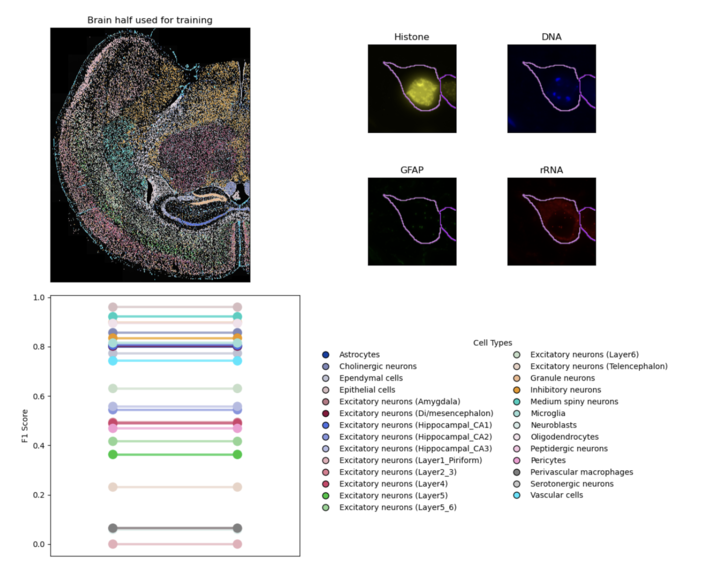
\includegraphics[width=.9\linewidth]{./figs/spatial.png}
\caption{\label{fig:spatial_omics}{[}PLACEHOLDER] Spatial omics analysis.}
\end{figure}
\section{Discussion}
\label{sec:orgf37b369}
While point-and-click interfaces open the world of image analysis to many researchers, they are not as effective for computational workflows with no human-in-the-loop. In this work we introduced our new library cp\_measure, which calculates a set of widely used engineered features relevant to whole images and to regions of interest (object masks). It enables simpler automated profiling of microscopy data in short scripts and complex pipelines. The modularity it provides facilitates pipelines with better scaling capabilities for high-content microscopy, with or without cloud infrastructure.

The biologically interpretable features provided by cp\_measure complement deep learning features and offer a better mechanistic understanding of the underlying biology. A potential workflow would be to use deep learning features to cluster and then use cp\_measure features from these clusters. As a whole, when used in tandem with generalist image-processing tools, such as Cellpose for segmentation \cite{stringerCellposeGeneralistAlgorithm2021}, machine and deep learning workflows can be streamlined. 

Already, Cellprofiler features have been used in multiple experiments, including in non-biological contexts such as environmental monitoring \citep{ideharaExploringNileRed2025}. By association, we foresee cp\_measure being useful for a broad scientific community beyond image-based profiling.
\section{Future work}
\label{sec:org5cdbb12}
We propose in future work to make it possible for CellProfiler to import cp\_measure, which offers several benefits. It would ensure that the results from pipelines built with either tool will always be comparable, while also providing the opportunity to formalize the inputs and outputs of all measurements. It would also mean that any changes made in cp\_measure propagate to CellProfiler, benefiting the community for which it was originally developed.

We also plan to develop a comprehensive test suite to guarantee mathematical correctness, which currently CellProfiler itself is lacking. A comprehensive test suite would enable more confident and expedient optimization for the most compute-consuming features, such as granularity, by providing rapid iteration capabilities. Once tests are in place, we could add support for just-in-time compiling and GPUs. We envision that cp\_measure could also be the place to develop and distribute new measurements from the community. 

\bibliographystyle{icml2025}
\bibliography{bibliography}
\section{Appendix}
\label{sec:orgdd18dd8}
\subsection{Methods}
\label{sec:orgb3e9382}
\subsubsection{Data and software}
\label{sec:orgbda0ae2}
The code for cp\_measure is available on \url{https://anonymous.4open.science/r/cp\_measure-B0DA}. All code to reproduce the analyses and figures, alongside links to the original data, is available on the GitHub repository \url{https://github.com/afermg/2025\_cpmeasure/}. The datasets we produced for this work are available on Zenodo, and the latest version can be found on \url{https://zenodo.org/records/15390631/latest}.
\subsubsection{Data and software}
\label{sec:acknowledgements}

This work was supported by GSK and the National Institutes of Health, grant (R35 GM122547 to AEC). The authors would like to thank Nodar Gogoberidze, Beth Cimini, Minh Doan and Eliot McKinley for their valuable feedback and discussions during the course of this project.
\end{document}
